\documentclass[11pt]{article}
\setlength{\oddsidemargin}{12pt}
\setlength{\textwidth}{6.5in}
\setlength{\textheight}{9in}
\pagestyle{empty}
\setlength{\parskip}{7pt plus 2pt minus 2pt}

\usepackage{graphicx}
\graphicspath{ {.} }

\begin{document}

    \begin{center}
    {{\large CS 230 : Discrete Computational Structures}}
        \\

%\vspace*{1cm}

        {\bf Spring Semester, 2021}\\

        {\sc Assignment \#11} {\bf [Extra Credit]}\\
        {\bf Due Date:} Friday, April 30
    \end{center}

    For the problems below, explain your answers and show your reasoning.

%\vspace*{0.5cm}

    \begin{enumerate}

        \item {\bf [10 Pts]} If $G$ is a simple graph with $n$ vertices and $n$ edges,
        is $G$ connected? If {\it yes}, give a short justification. If {\it no}, give
        a counterexample. \\
        No. Consider this beautifully drawn graph as a counter example: \\
        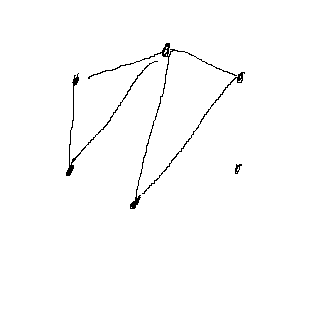
\includegraphics{graph.png}


        \item {\bf [8 Pts]} Consider a graph $G$ that has 7 vertices with degrees of 5, 4, 3, 3, 2, 2, 1. How many edges does $G$ have? Explain. \\
        By the Handshake Theorem: $(5+4+3+3+2+2+1)/2 = 10$ edges.

        \item {\bf [12 Pts]} Prove by induction that a complete binary tree of height $h$ has $2^h$ leaves. Use the inductive definition of complete binary trees.
        \begin{enumerate}
            \item Base Case: A complete binary tree of height 0 has 1 leaf node $2^0$. The CBT of height $0 + 1 = 1$ will have 2 leaves because by def of CBT's, the CBT of the next height will fill the left and right subtrees of all the current leaves. The \# of leaves will double for every increase in height by 1. So, $2^0*2 = 2^1$
            \item IH: A CBT of height k has twice the leaves of a CBT with height $k - 1$. So, $2^{k - 1}*2 = 2^k$ leaves
            \item Prove: CBT's of height $(k + 1)$ has twice the leaves of a CBT of height $(k + 1) - 1 = k$
            \item By IH, tree of height k has $2^k$ leaves
            \item $n^{k} * 2 = n^{k+1}$ \null\hfill QED
        \end{enumerate}

        \item {\bf [20 Pts]} Prove that a graph is a tree if and only if it is acyclic but adding any edge will create a cycle.


    \end{enumerate}

\end{document}

